% Waiting-vs-revision frontier, ScanNet200 val (312 scenes).
% ---------------------------------------------------------------------------
% PROVENANCE (read before editing):
%   Run     : audit/indoor_provretro/  (one streaming pass, all arms derived
%             from it; gate points recomputed from the same event log)
%   Numbers : frontiers.json, scannet_provisional_summary.json
%   Cache   : audit/indoor_n_sweep/mask3d_cache, manifest sha256 4428c7b7...,
%             verified byte-identical before and after the run.
%   H=inf is deliberately NOT plotted: it is a retrospective bound, not an
%   operating point. It is in the supplement table (tab:provretro-supp).
%   lsc_provisional(H) == lsc_gate(N=H+1) is an IDENTITY, verified 312/312
%   scenes. Do NOT redraw or recaption this as provisional beating
%   confirmation on consistency.
% ---------------------------------------------------------------------------
\begin{figure}[tb]
\centering
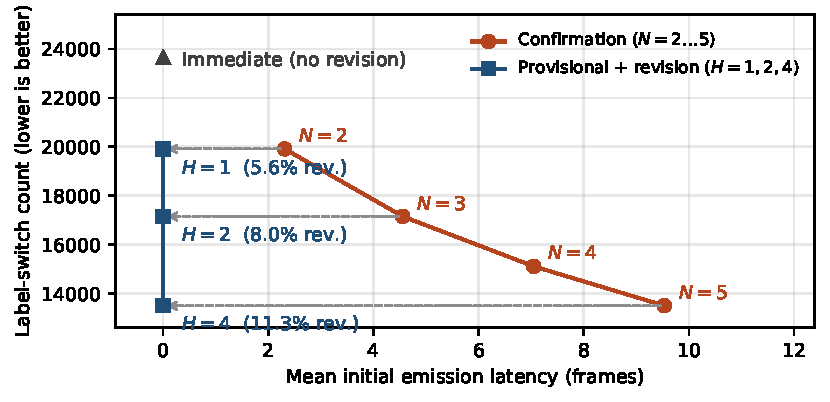
\includegraphics[width=\linewidth]{figs/fig_provretro_frontier.pdf}
\caption{\textbf{Waiting versus revision} on ScanNet200 val.
Confirmation ($N{=}2{\ldots}5$) buys fewer label switches with pre-emission
latency; provisional emission at revision horizon $H$ reaches the same switch
counts at zero latency, paying revisions instead (annotated). Arrows join the
definitionally paired settings: the retrospectively finalised label at horizon
$H$ \emph{is} the emitted label of the $(H{+}1)$-th observation, so $H$ and
$N{=}H{+}1$ have identical switch counts by construction, not by measurement.
All points come from one pass over the same frozen proposals, so counts differ
slightly from Tab.~\ref{tab:indoor}; per-arm counts and the $H{\to}\infty$
bound are in Tab.~\ref{tab:provretro-supp}.}
\label{fig:provretro}
\end{figure}
